% Template for a Thesis
%
% 6-results.tex
%
% Results

\chapter{Results}\label{ch:results}

This chapter shows the results for each section of the development of this thesis, ranging from score plots for BPE alignments, to algorithm runtimes. The scores display four different metrics, which have been explained previously in the Translation chapter.~\ref{tra:metrics}

\section{Replication of BPE}

The results for BPE show that in the case of Fastalign, where the baseline F1 score is 0.6, and the best BPE result is with 1000 BPE merges, and a F1 score of 0.609.

\begin{figure}[!ht]
    \centering
    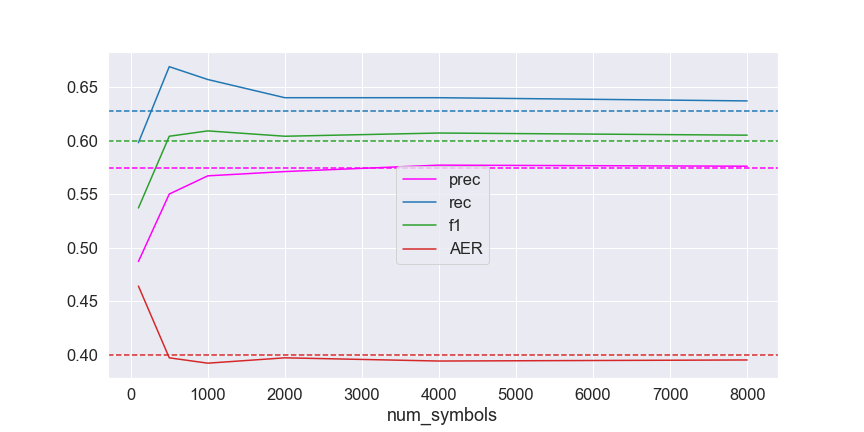
\includegraphics[width=12cm]{../reports/scores_normal_bpe/eng_deu_fastalign.png}
    \caption{Scores of BPE over baseline, using Fastalign}
\end{figure}

In the case of Eflomal, the baseline F1 score is 0.72, and the best BPE result is for 6000 BPE merges with a F1 score of 0.701. In absolute terms, BPE units using Eflomal have an absolute higher score than BPE units using Fastalign. But these values only make sense when compared against the baseline.

\begin{figure}[!ht]
    \centering
    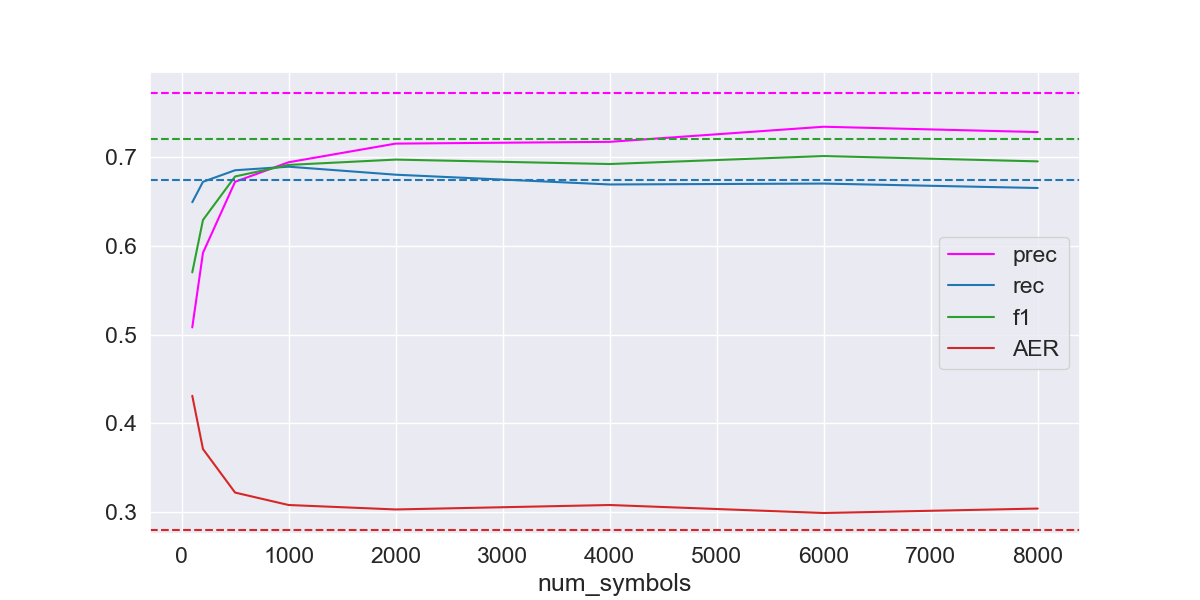
\includegraphics[width=12cm]{../reports/scores_normal_bpe/eng_deu_eflomal.png}
    \caption{Scores of BPE over baseline, using Eflomal}
\end{figure}

The alignment algorithms, Fastalign and Eflomal, require one language to be given as source and the other as target, and perform the alignment based on this. Throughout the thesis, English has been taken as the source language and German as the target. It might have been interesting to see that swapping the languages would yield different results, by swapping the languages in the global variables file. The difference between these two cases is barely perceptible, 0.03\% across all numbers of merges. Therefore, it is assumed that swapping the source and target language has no effect in the experiment result scores.

\section{Replication of BPE dropout}

When getting BPE dropout results, the desired comparison is that of BPE dropout with respect to BPE. As a result, the BPE scores are taken as baseline, instead of the gold standard scores as in the previous case. As explained in the Methodology chapter~\ref{met:replbpedrop}, the BPE dropout pipeline is run a number of times, resulting in many alignment files. Out of these, three types of results are obtained: union, intersection and threshold.

\begin{itemize}
	\item The \textbf{union} case takes all alignments into account, which results in a big list of alignments per sentence. These will most probably include the correct alignments, but there will many other wrong alignments. This case has low precision and high recall.
	\item The \textbf{intersection} case takes only those alignments which are present in all alignment files, resulting in a few number of alignments per sentence. Most probably, these alignments will be correct. But there will also be many alignment smissing. This case has high precision and low recall.
	\item The \textbf{threshold} case is a mixture between the previous two cases. Given a threshold, for instance 0.7, an alignemnt is accepted if it is present in 70\% of the alignment files. Smaller values for this variable resemble the union case, since more alignments are accepted. Higher threshold numbers resemble the intersection case, where alignments must be present in more and more files in order to be accepted.
\end{itemize}

The following figures show the results for a \emph{dropout} value of 0.1 or 10\%, and the union, intersection and threshold cases.

 \begin{figure}[!ht]
     \centering
     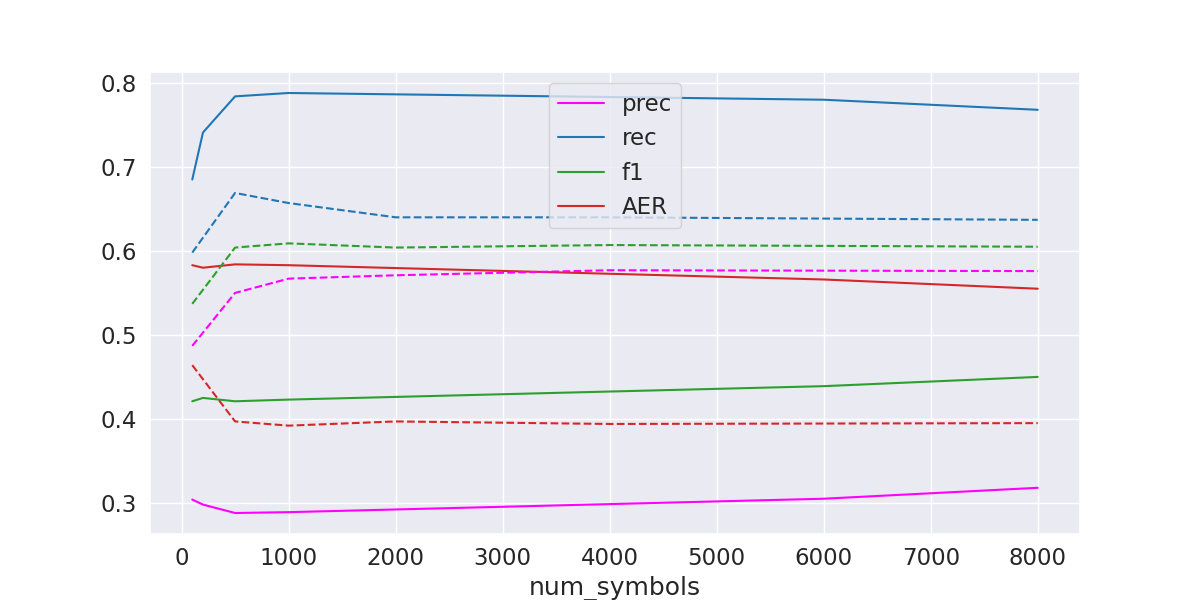
\includegraphics[width=12cm]{../reports/scores_dropout_bpe/space/0.1/union_fastalign.png}
     \caption{Scores for BPE with dropout 0.1, union mode}
 \end{figure}
 
 \begin{figure}[!ht]
     \centering
     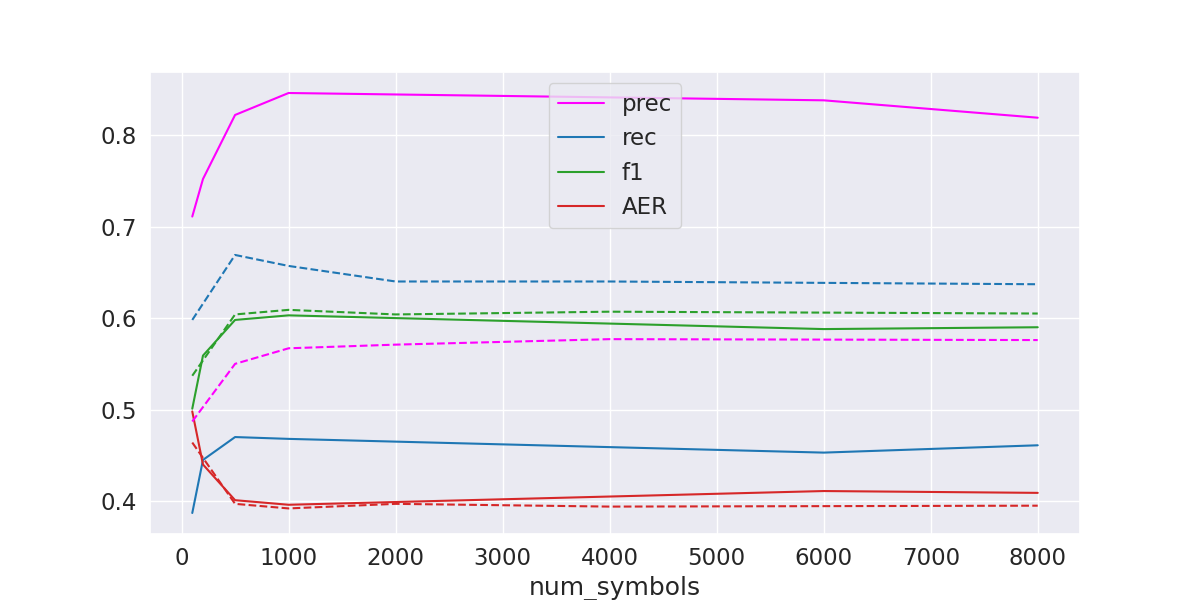
\includegraphics[width=11.5cm]{../reports/scores_dropout_bpe/space/0.1/inter_fastalign.png}
     \caption{Scores for BPE with dropout 0.1, intersection mode}
 \end{figure}

It can be seen that the F1 score improves consistently the more BPE units have been merged. Since there are more merges, there are fewer units, most words are completely merged and the uncertainty of aligning BPE units is lower, since the sentence looks more and more similar to the raw sentence where there are just words. Regarding the threshold case, the following two figures show the scores for threshold 0.3 and 0.7, which achieves the best F1 score, namely 0.635.

\begin{figure}[!ht]
    \centering
    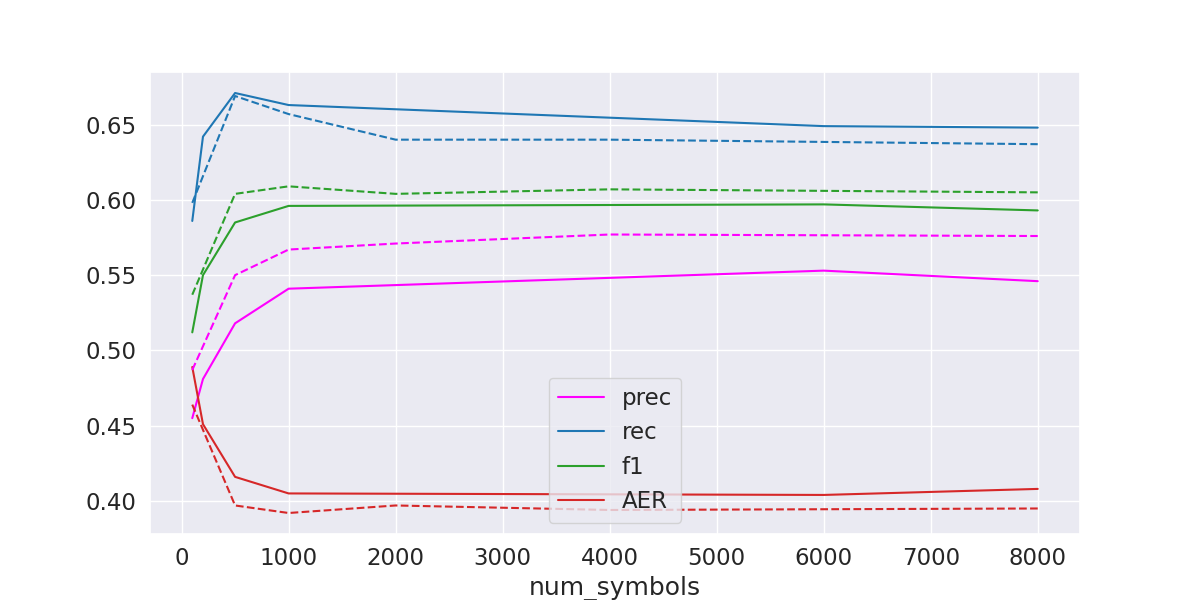
\includegraphics[width=11.5cm]{../reports/scores_dropout_bpe/space/0.1/0.3_thres_fastalign.png}
    \caption{Scores for BPE with dropout 0.1, threshold mode at 0.3}
\end{figure}

\begin{figure}[!ht]
    \centering
    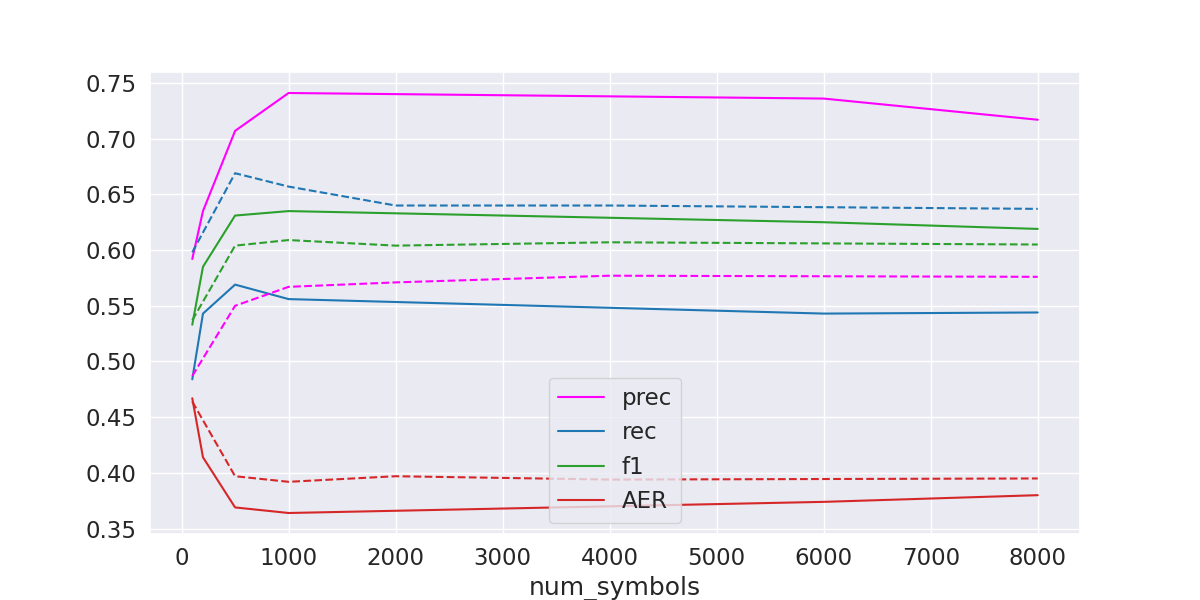
\includegraphics[width=11.5cm]{../reports/scores_dropout_bpe/space/0.1/0.7_thres_fastalign.png}
    \caption{Scores for BPE with dropout 0.1, threshold mode at 0.7}
\end{figure}

As the BPE dropout paper states~\cite{provilkov2019bpedropout}, BPE dropout improves BPE consistently no matter how many merges are performed. 

